\documentclass[a4paper]{report}
\usepackage[T1]{fontenc}
\usepackage[utf8]{inputenc}
\usepackage[english]{babel}
\usepackage{titlesec}
\usepackage{lipsum}
\usepackage{booktabs}
\usepackage{hyperref}
\usepackage{graphicx}
\usepackage{float}
\usepackage{rotating}
\usepackage[dvipsnames]{xcolor}
\usepackage{enumerate}
\usepackage[shortlabels]{enumitem}
\usepackage{geometry}
\usepackage{pdflscape}
\usepackage{caption}
\usepackage{afterpage}
\graphicspath{{./img/}}

\begin{document}


\titleformat{\chapter}[hang] 
{\normalfont\huge\bfseries}{\thechapter}{1em}{} 

\title{e-Mobility for All}
\author{Enrico Brunetti, Matteo Gionfriddo}
\date{date} %%TODO

\begin{titlepage}
\begin{figure}[t]
\centering
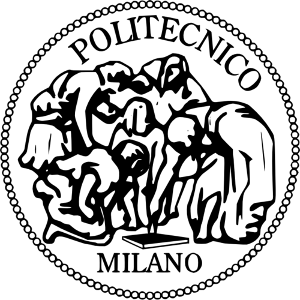
\includegraphics[width=0.3\textwidth]{Logo}
\end{figure}
\begin{center}
    \textsc{ \LARGE{Politecnico di Milano \\}}
	\textsc{ \Large {School of Industrial and Information Engineering\\ }}
	\vspace{3mm}
	\textnormal{ \Large{Software Engineering 2 Project\\}}
	\vspace{30mm}
	\fontsize{10mm}{7mm}\selectfont 
    \textup{e-Mobility for All}\\
    \textnormal{ \LARGE{Design Document\\}}
\end{center}

\vspace{18mm}

\begin{center}
    \textnormal{\large{\bf Authors:\\}}
	{\large Enrico Brunetti \\ Matteo Gionfriddo }
	\fontsize{10mm}{5mm}\selectfont 
\end{center}
\vspace{15mm}

\centering{\large{
Academic Year 2022/2023 \\
\vspace{10mm}
Milano, -/12/2022 \\
\vspace{2mm}
Version 1.0
}}

\end{titlepage}

\newgeometry{top=3cm}
\tableofcontents
\listoffigures
\begingroup
\let\clearpage\relax %avoid to put it on a new page
\listoftables
\endgroup
\restoregeometry

\chapter{Introduction}
\section{Purpose}

The purpose of this document is to detail the design of the software and of the architecture regarding the system of
eMall. The analysis has been made in a more detailed approach for the description of each component
and the overall architecture of the system, by also covering the relationships between each of them. Furthermore has been inserted mockups of User and Web interfaces and a plan for the implementation,
testing and integration of the system..

\section{Scope}
\textit{eMall} is an application system designed for help End-Users to take advantage of the services for charging electric vehicles and helps Charging Point Operators manage associated charging
stations.\\
The End-Users can use the mobile app to browse a map that displays the charging stations nearby, their cost and any special offer they have and book and use an electric vehicle charge.\\
The CPO Workers can use the web application to manage their associated charging stations and interact with DSO in order to acquire energy furniture. The system is supported by APIs provided by a map service and suited for interaction between the various providers (eMSPs, CPOs, and DSOs) as explained in the RASD and in the following sections of this document.
\section{Definitions,Acronyms,Abbreviations}
\begin{itemize}
\item \textit{API}: Application Programming Interface.
\item \textit{DBMS}: Database Management System.
\item \textit{eMSP}: e-Mobility Service Provider.
\item \textit{CPO}: Charging Point Operator.
\item \textit{CPOW}: Charging Point Operator Worker.
\item \textit{CPMS}: Charge Point Management System.
\item \textit{DSO}: Distribution System Operator.
\end{itemize}
\section{Revision history}
\begin{itemize}
\item |-12-2022 Version 1.0.
\end{itemize}
\section{Reference Documents}
\begin{itemize}
\item Assignment Document "Assignment RDD AY 2022-2023\_v3.pdf"
\item RASD Document "RASD1.pdf"
\end{itemize}
\section{Document Structure(TO DO)}

\chapter{Architectural Design(TO BE BETTER EDITED FROM THE ORIGINAL DOCUMENT)}
\section{Overview:}
The application will be developed using the client-server paradigm on a three-tiered architecture. The three layers of the application (Presentation, Application and Data) are divided into clusters of machines (i.e. tiers) that actually cooperate to provide a specific functionality. In this case we have three tiers  and each tier is responsible for one of the three layers. The client tier is responsible for the \textbf{Presentation} layer; therefore, in this architecture, are included eMPS and CPMS applications. The UIs provided are just meant to show results and to allow clients to choose what they want. In particular there are two types of clients: a \textbf{mobile app} for the End-Users which use it to book and take advantage of electric vehicle charges, directly connected to the associated eMSP and a  \textbf{web app} for CPOWs for managing associated charging stations, directly connected to the related CPMS. \\
The Application tier takes care of the application layer encapsulating all is needed concerning the application logic. It receives the requests from the clients and handles them. It's also responsible for sending asynchronous notifications to a CPMS (which can be forwarded to an End-User trough eMSP APIs) in the presentation layer when certain conditions are met.\\
The \textbf{Application} tier communicates with the \textbf{Data} tier, responsible for the Data Access layer, that is the layer responsible for accessing the DataBases and performing queries on them.
\section{Component view}
In the figure \ref{fig:general-component-diagram} the \textit{Component Diagram} for the \textit{eMall} system is reported. This is a high level view in which only the main components are immediately shown, while some components will be better detailed afterwards.

\begin{figure}[hp]
\centering
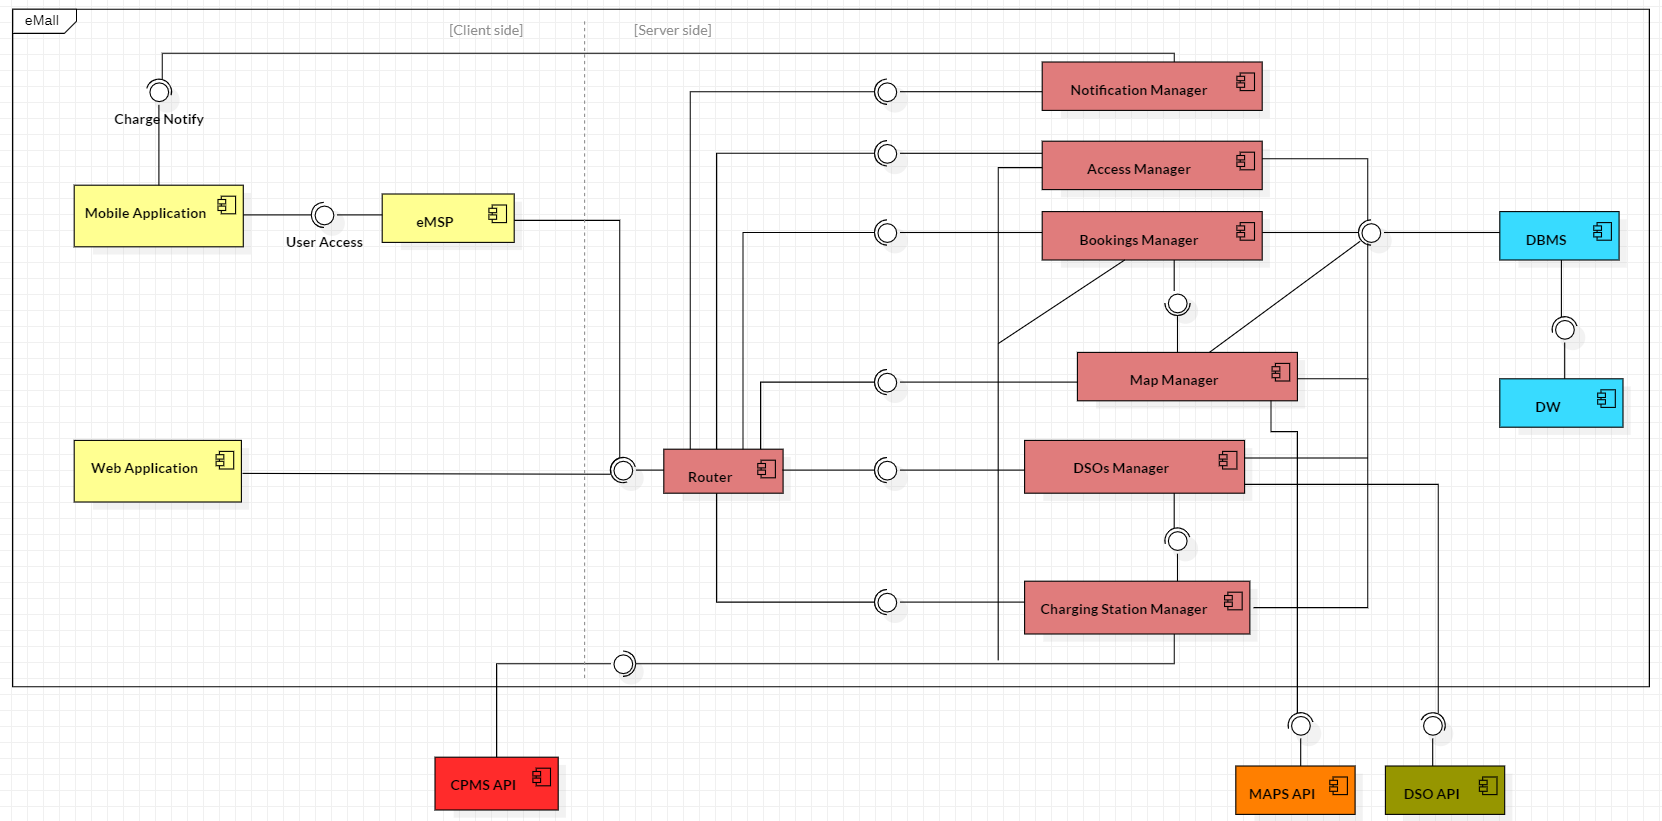
\includegraphics[scale=0.5 ]{img/GENERAL DIAGRAM_v2.png}
\caption{UML Component Diagram}
\label{fig:general-component-diagram}
\end{figure}


\begin{figure}[hp]
\centering
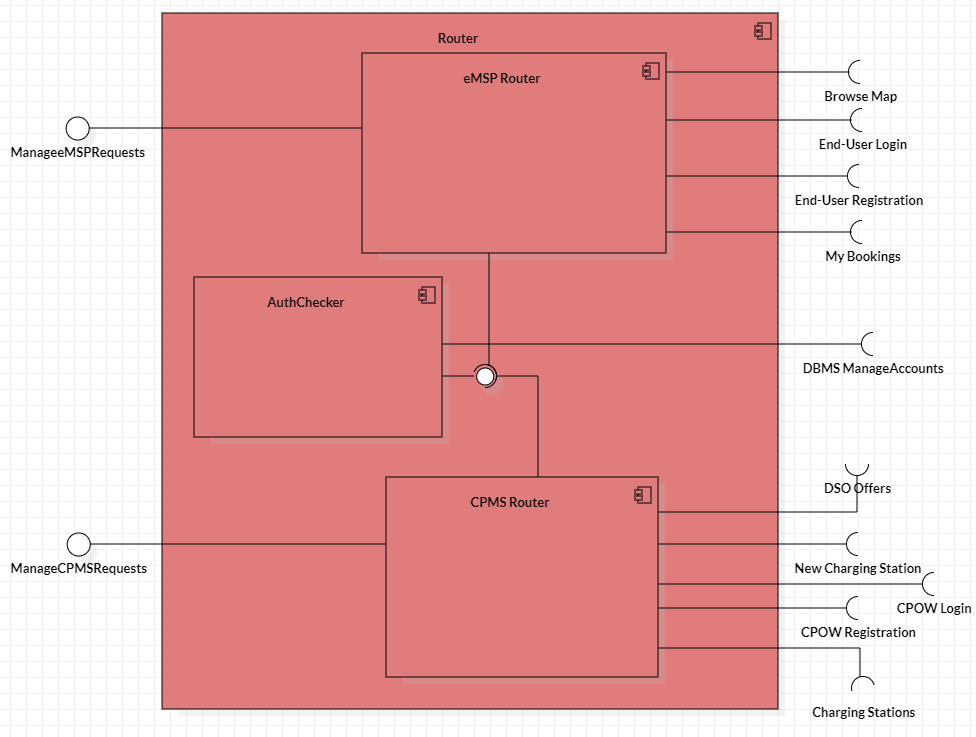
\includegraphics[scale=0.6]{img/ROUTER.png}
\caption{UML Component Diagram for \textit{Router} component}
\label{fig:router-component}
\end{figure}

In this diagram when two components can communicate using different interfaces a single interface link is 
reported, for the sake of readability. The various components are now described and detailed:
\begin{itemize}
\item \textbf{Router}: it has the role of dispatching the requests coming from the users applications. Before doing this it has also the important role of verifying the user authentication. In figure \ref{fig:router-component} a more detailed view is provided, putting in evidence the various interfaces for the eMSP and CPMS side.

\item \textbf{BookingsManager}: this component is in charge of all concern the management of the bookings associated to the End-Users. It permits to make a new booking or retrie all personal bookings from the database trough the \textit{DBMS} component and proceed from one of them with the charging process (trough an interface directly connected to an CPMS). This component is described in figure \ref{fig:bookingsmgr-component} .


\begin{figure}[htp]
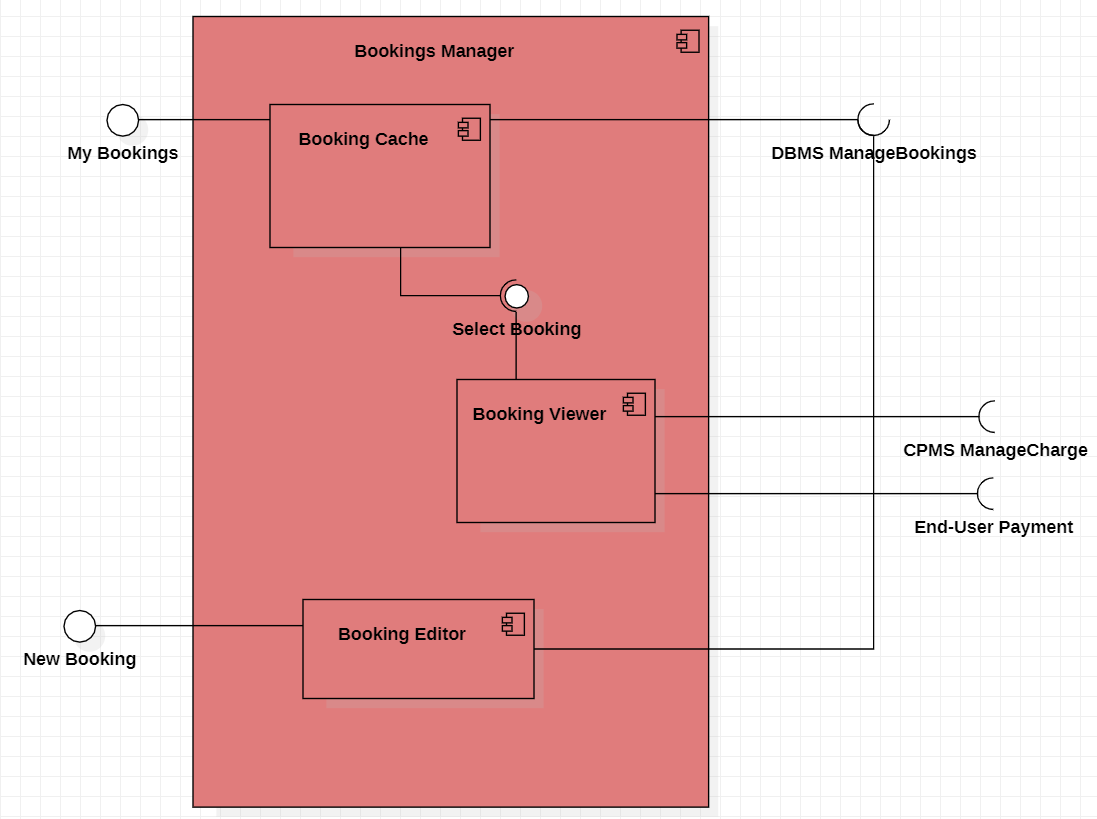
\includegraphics[scale=0.6]{img/BOOKINGS MANAGER.png}
\caption{UML Component Diagram for \textit{BookingsManager} component}
\label{fig:bookingsmgr-component}
\end{figure}

\item \textbf{AccessManager}: it manages everything about registration and login of the users. He stores the accounts data through the \textit{DBMS} component and calls it also to verify the correctness of the login credentials. This component is detailed in figure \ref{fig:accessmgr-component}.

\begin{figure}[htp]
\centering
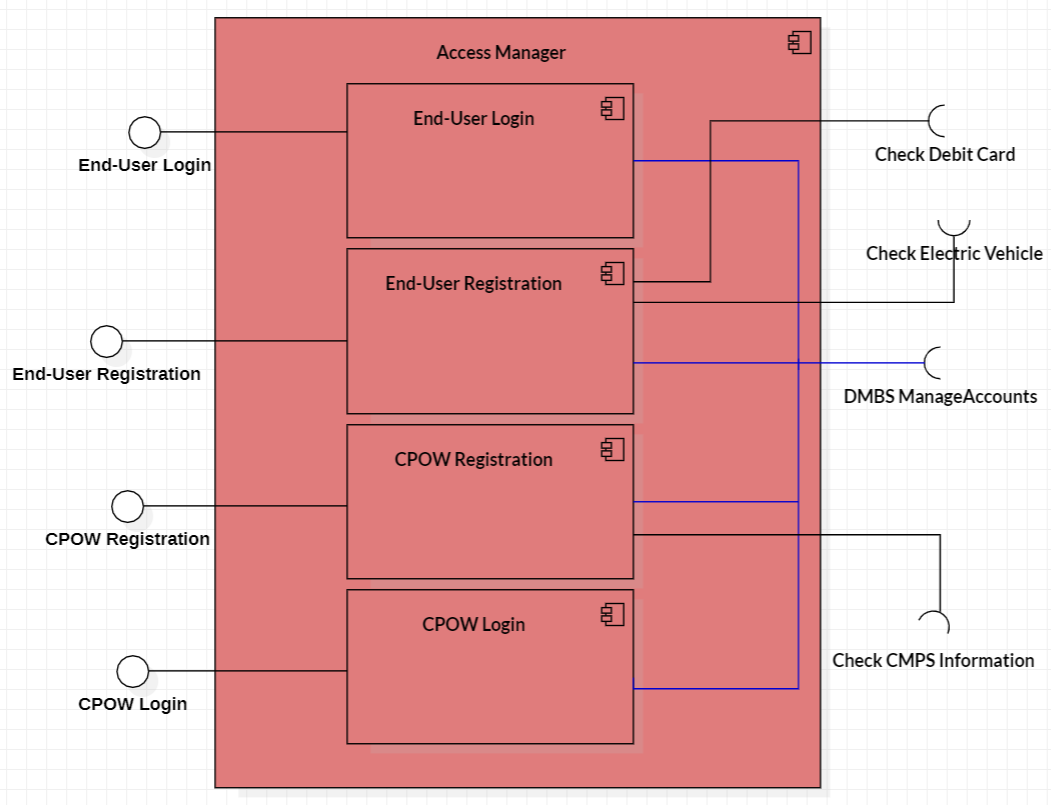
\includegraphics[scale=0.45]{img/ACCESS MANAGER.png}
\caption{UML Component Diagram for \textit{AccessManager} component}
\label{fig:accessmgr-component}
\end{figure}

\item \textbf{ChargingStationsManager}: it permits to view all charging stations associated to a certain CPMS and do all management operations for each one of them. It requires to communicate, by some interfaces, with the \textit{DBMS} component and the associated CPMS. It is shown in the diagram in figure \ref{fig:chargingstationsmgr-component}.


\begin{figure}[htp]
\centering
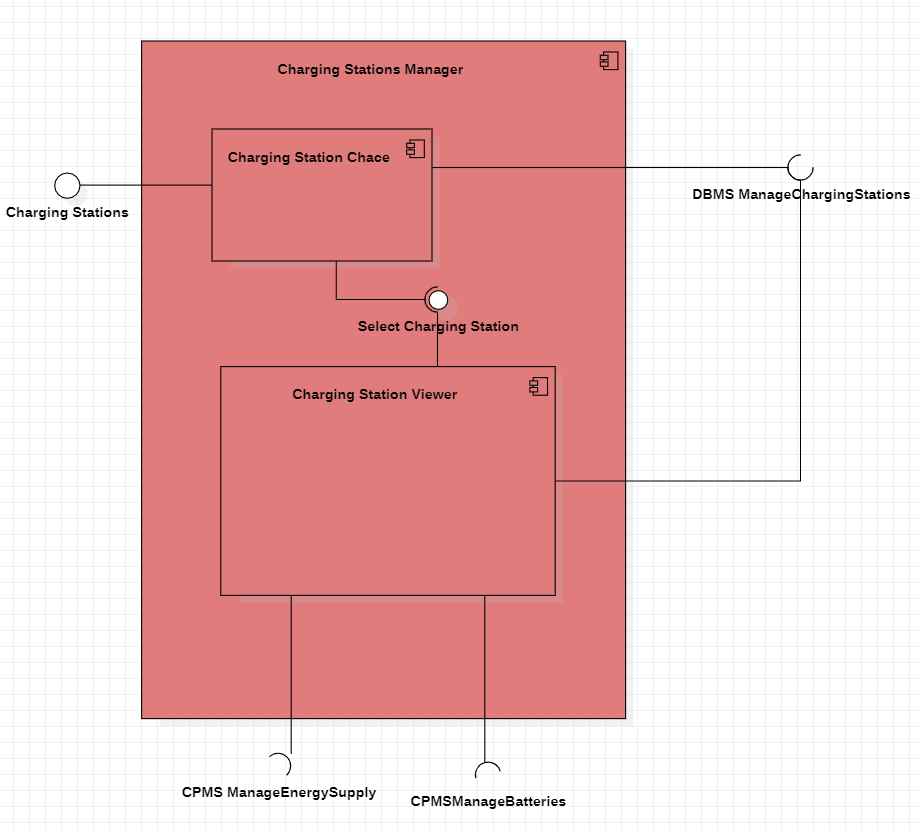
\includegraphics[scale=0.6]{img/CHARGING STATION MANAGER.png}
\caption{UML Component Diagram for \textit{CharginStationsManager} component}
\label{fig:chargingstationsmgr-component}
\end{figure}

\item \textbf{NotificationManager}: TO DO.

\item \textbf{DBMS}: this component manages the operational database.

\item \textbf{DataWarehouse}: TO DO .

\item \textbf{DSOAPI}: this is an external component, managed by the DSO (an instance for each of them which supports the system), whose interface is standardized as described in the \textit{Components Interfaces} section. It is necessary in order to retrieve prices and offers of energy furniture provided by the different companies.

\item \textbf{MapsAPI}: this is an external component which is exploited to obtain maps, which will be shown when browsing charging stations map.

\item \textbf{CPMSAPI}: TO DO.

\item \textbf{eMSP}: TO DO.

\item \textbf{MobileApplication}: this component entirely resides in the \textit{Presentation layer} and it's just an interface to allow the users to take advantage of the services offered by eMSP on their mobile devices, such that view nearby charging stations offers and book and use electric vehicle charges.

\item \textbf{WebApplication}: this component is the \textit{Presentation layer} of the web app which allows CPOW to interact with his associated CPMS in order to take management decision of the related charging stations.
\end{itemize}

\section{Deployment view}

So far, only an abstract and general view of the system has been provided. In this section a better detailed view of the system shows how the component previously described are actually deployed in different machines and how each tier is organized.
In figure \ref{fig:deployment-diagram} there is an UML Deployment Diagram which shows the allocation of the software components in the physical tiers of the system. 

\begin{figure}[htp]
\centering
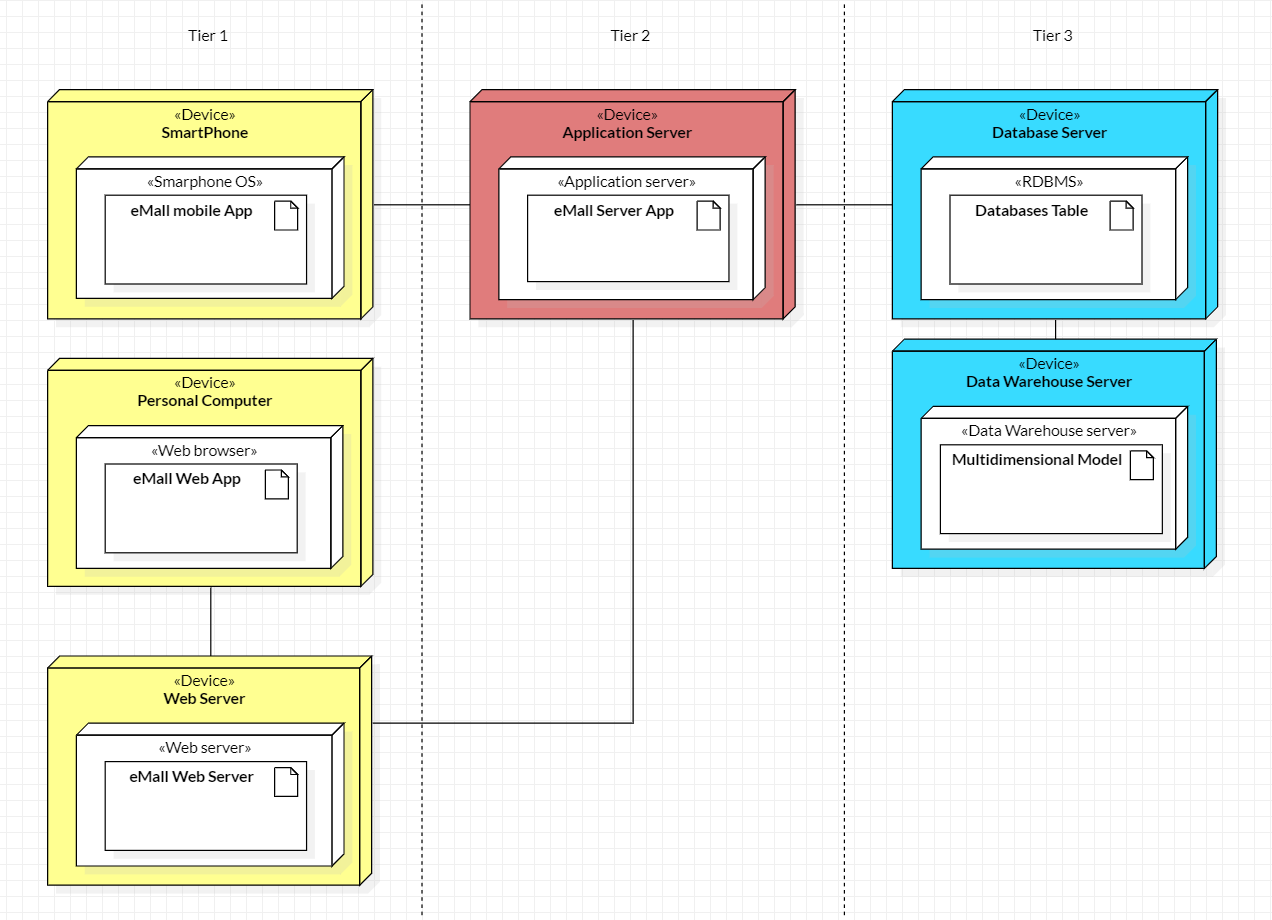
\includegraphics[scale=0.6]{img/DEPLOYMENT DIAGRAM.png}
\caption{UML Deployment Diagram}
\label{fig:deployment-diagram}
\end{figure}

W.r.t to the component diagram (figure \ref{fig:general-component-diagram}), the different colors indicate the allocation of components.
For the presentation tier clearly the \textit{smartphones} contain the \textit{MobileApplication} while the \textit{personal computers} and the \textit{web server} contain the \textit{Web Application}.\\
All application logic components (orange in the \textit{Component Diagram}) are deployed on the \textit{Application Server}, while the \textit{DBMS} component is deployed on the \textit{DataBase server} and the \textit{DataWarehouse} component is deployed on the \textit{DataWarehouse server}.

In the \textit{Mobile Application} case the client contains all the \textit{presentation layer} while in the \textit{Web Application} case the layer is splitted between the \textit{Web App} and the \textit{WebServer}; the \textit{WebServer} is responsible for contacting the application server and forward the client requests and responses.\\

\section{Runtime view}

\chapter{User interface design}
In this chapter are presented mobile application and web application mockups.

\begin{figure}[hp]
\centering
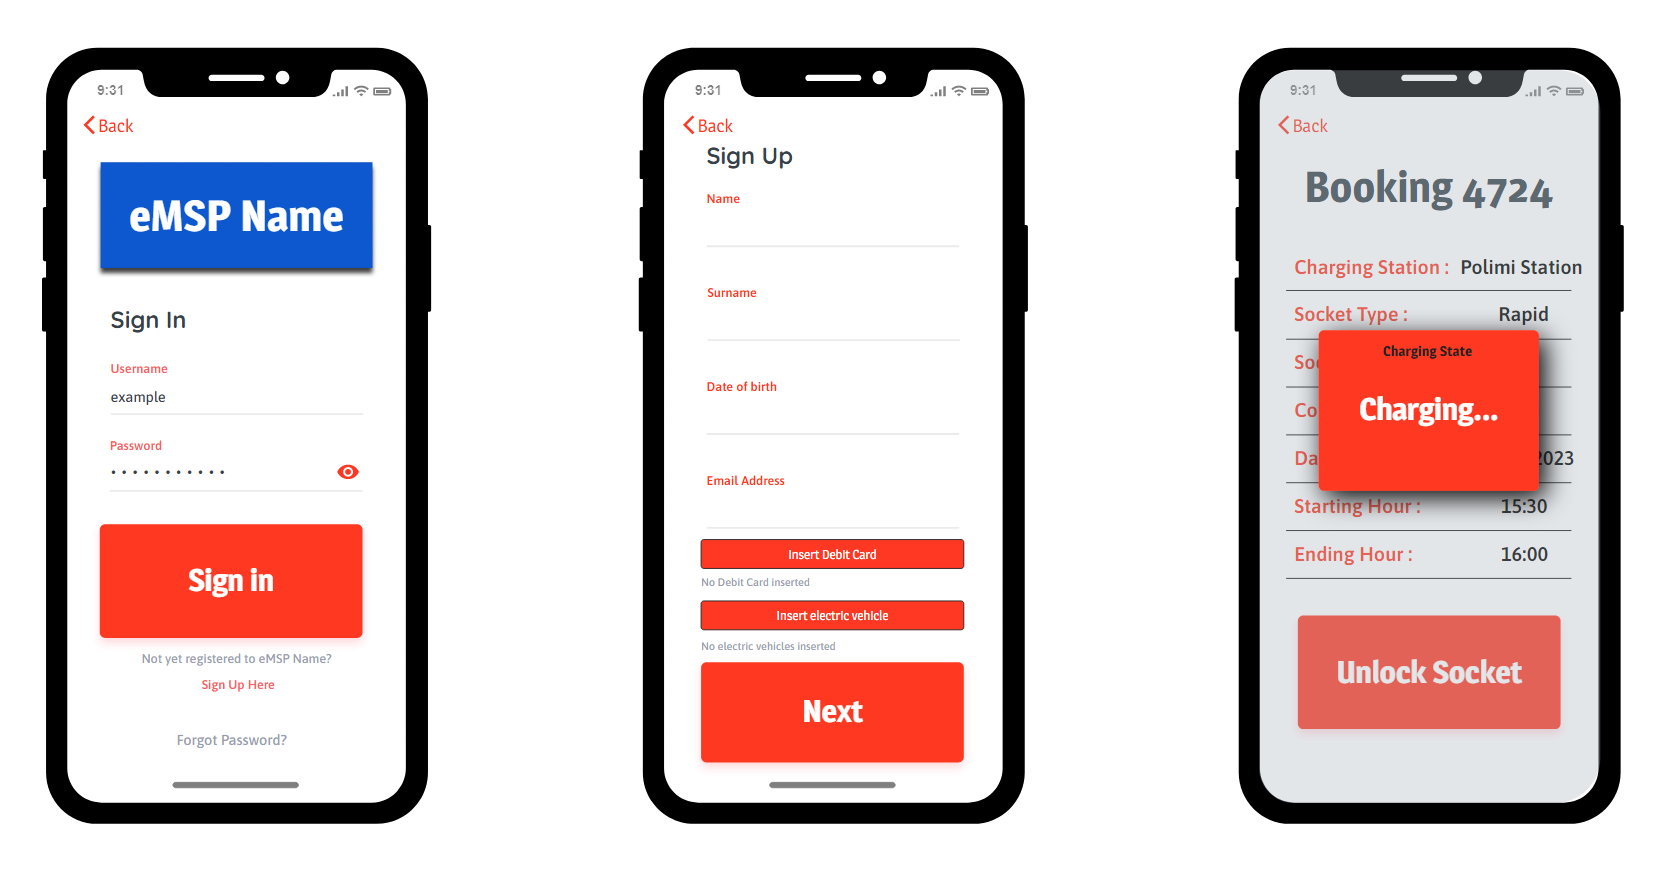
\includegraphics[scale=0.45]{img/mockups/MCKP1.png}
\caption{Mobile Application Mockups for End-User Log in, End-User Registration and Vehicle Charging State Popup Screens}
\label{fig:MobileApp-activity}
\end{figure}

\begin{figure}[hp]
\centering
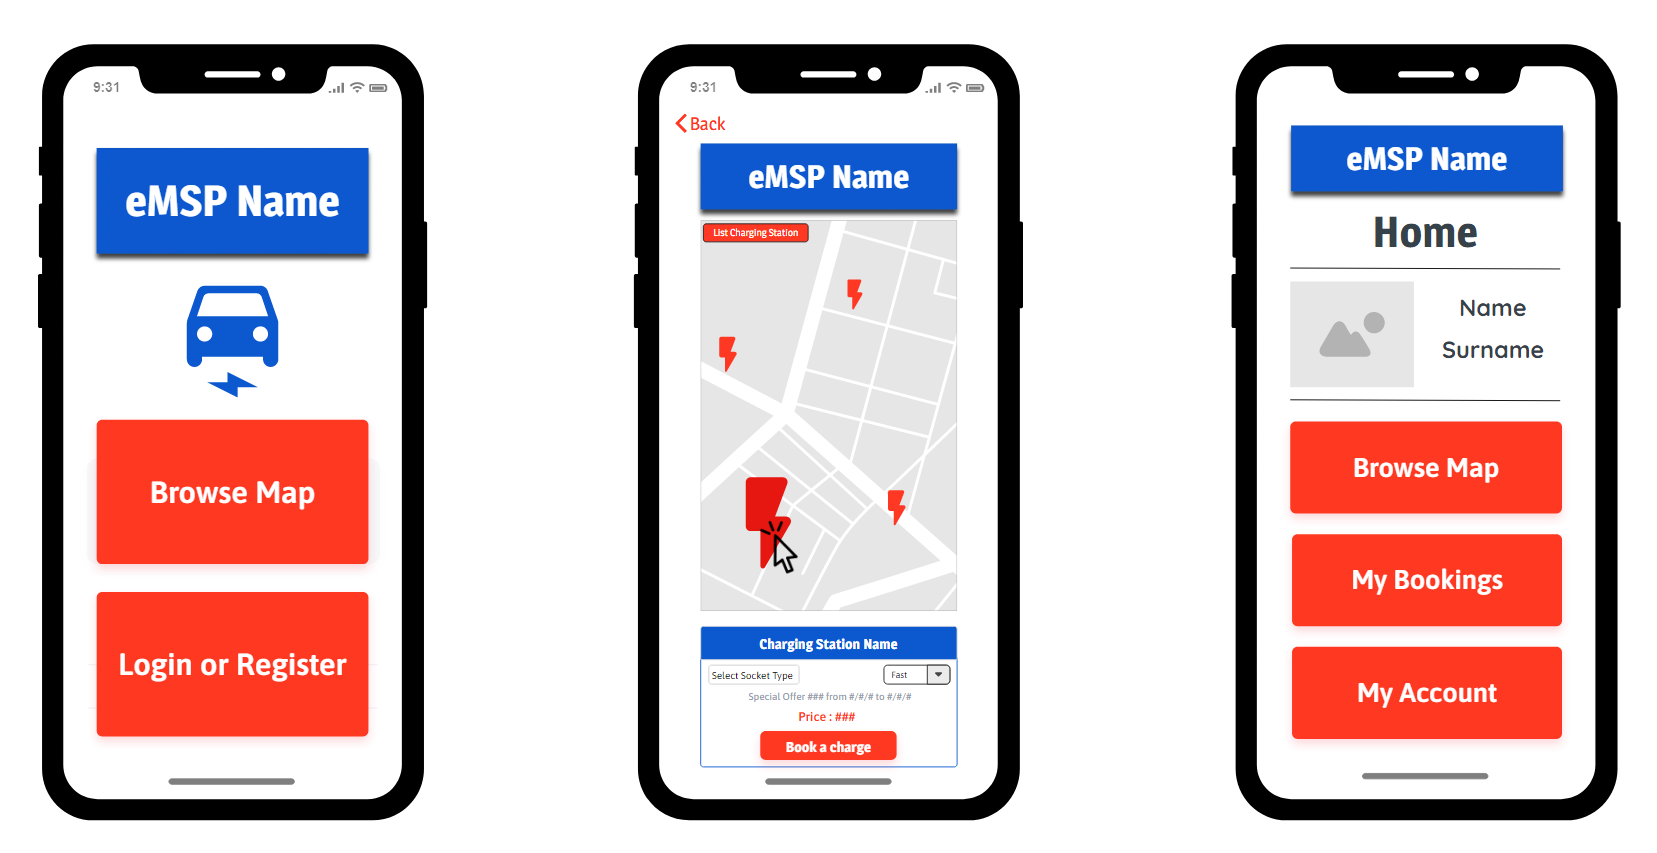
\includegraphics[scale=0.45]{img/mockups/MCKP2.png}
\caption{Mobile Application Mockups for Home Page, Charging Stations Map and Personal Home Page Screens}
\label{fig:MobileApp-activity}
\end{figure}

\begin{figure}[hp]
\centering
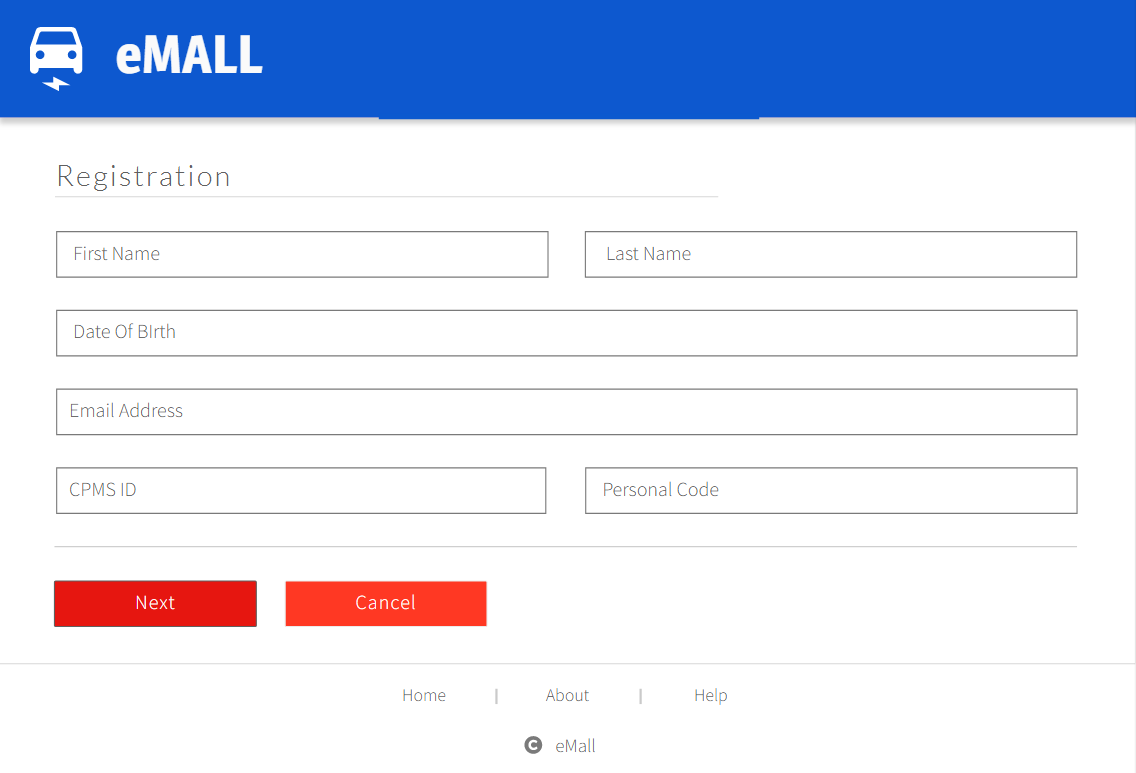
\includegraphics[scale=0.6]{img/mockups/MCKP_CPOWRegistration.png}
\caption{Web Application Mockup for CPOW Registration Screen}
\label{fig:MobileApp-activity}
\end{figure}


\begin{figure}[hp]
\centering
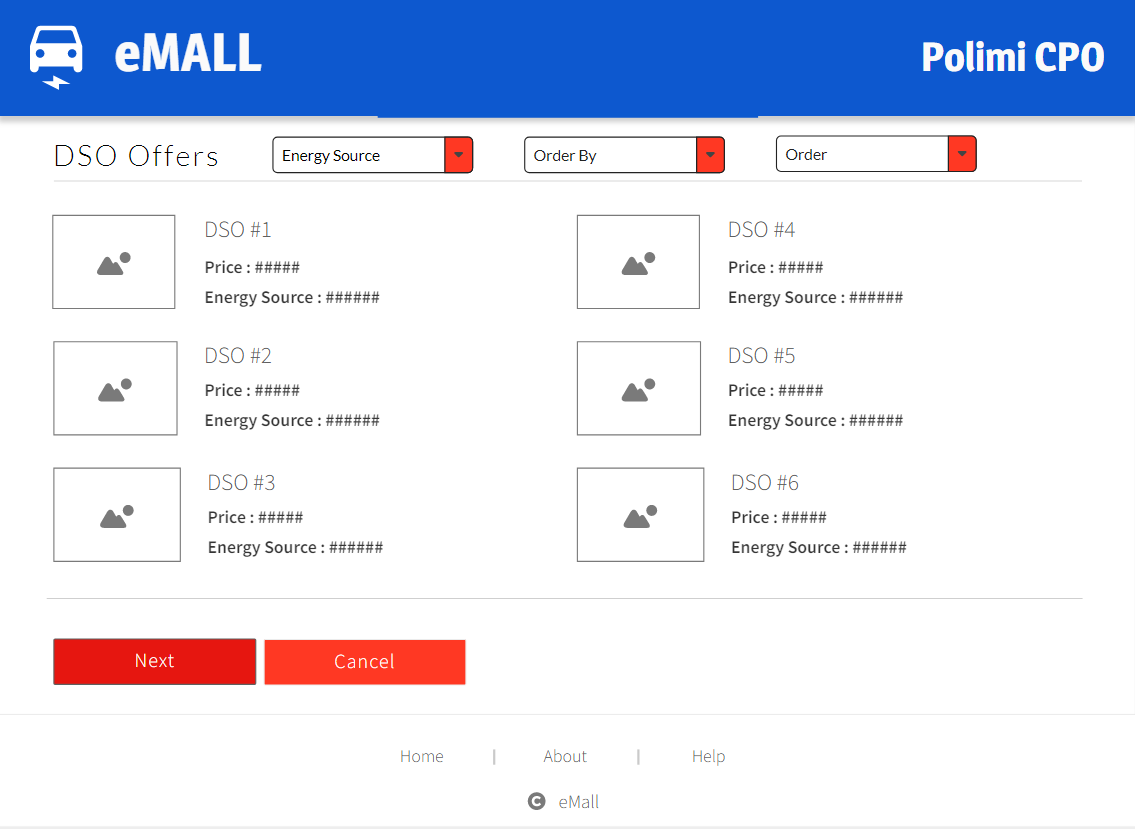
\includegraphics[scale=0.6]{img/mockups/MCKP_DSOoffers.png}
\caption{Web Application Mockup for DSO Offers Screen}
\label{fig:MobileApp-activity}
\end{figure}


\begin{figure}[hp]
\centering
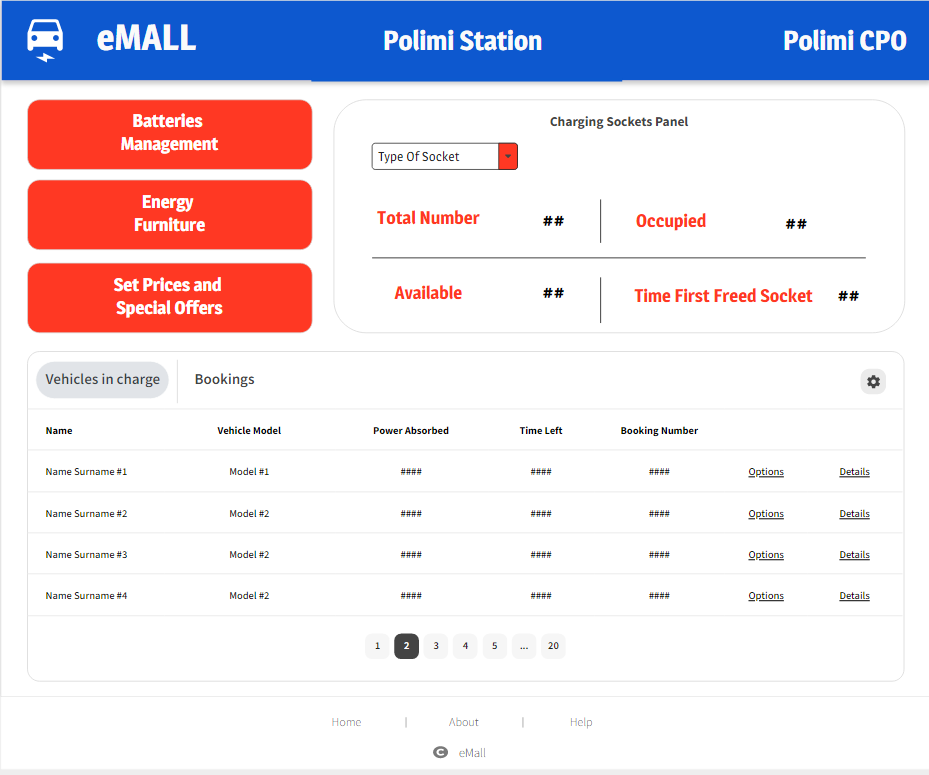
\includegraphics[scale=0.6]{img/mockups/MCKP_SelectedChargingStation.png}
\caption{Web Application Mockup for Selected Charging Station Screen}
\label{fig:MobileApp-activity}
\end{figure}

In the figures \ref{fig:MobileApp-activity}, \ref{fig:SupWebApp-activity}  are shown activity diagrams that describe how a End-User can navigate in the UIs offered by the application. Notice that  End-Users can quit the application from any state to reach the end state of the diagrams. No end state is represented and so are all the arrows that lead to them; this has been done for the sake of readability of the diagrams.

\afterpage{
\begin{landscape}
\begin{figure}[hp]
\centering
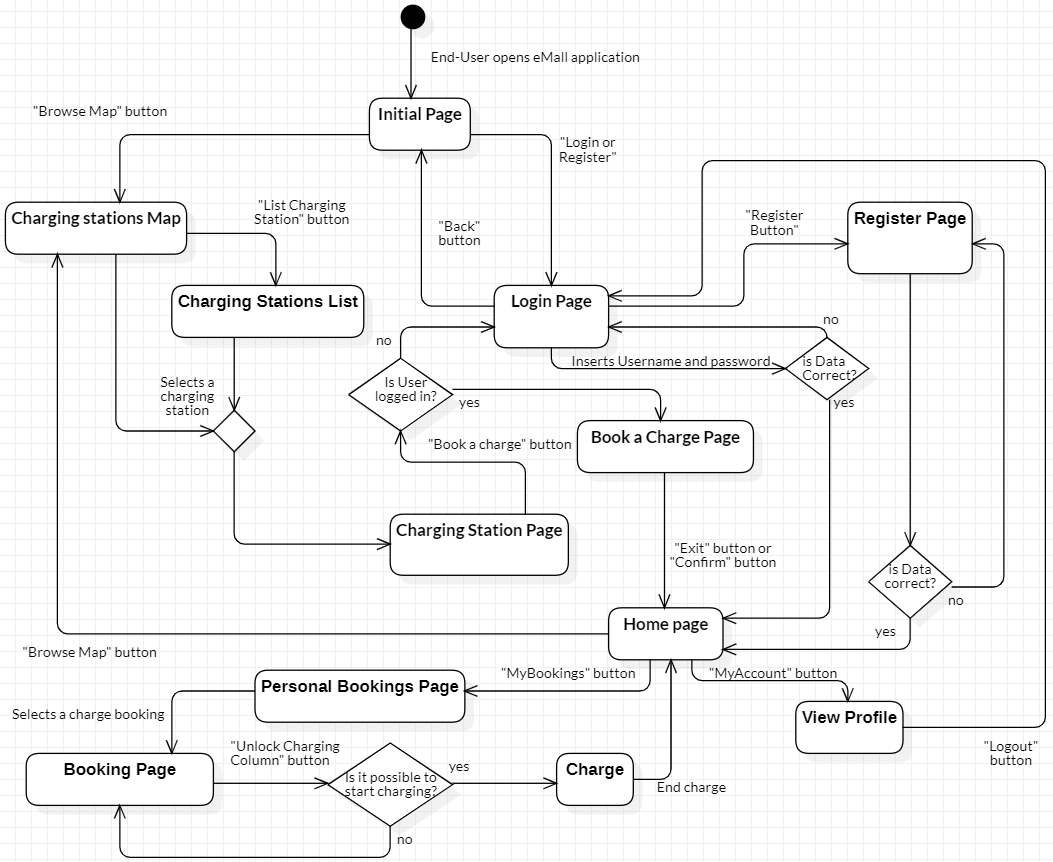
\includegraphics[scale=0.9]{img/ACTIVITY DIAGRAM END-USER.png}
\caption{UML Activity Diagram for the End-User Mobile App navigation}
\label{fig:MobileApp-activity}
\end{figure}
\end{landscape}

\begin{landscape}
\centering
\begin{figure}[hp]
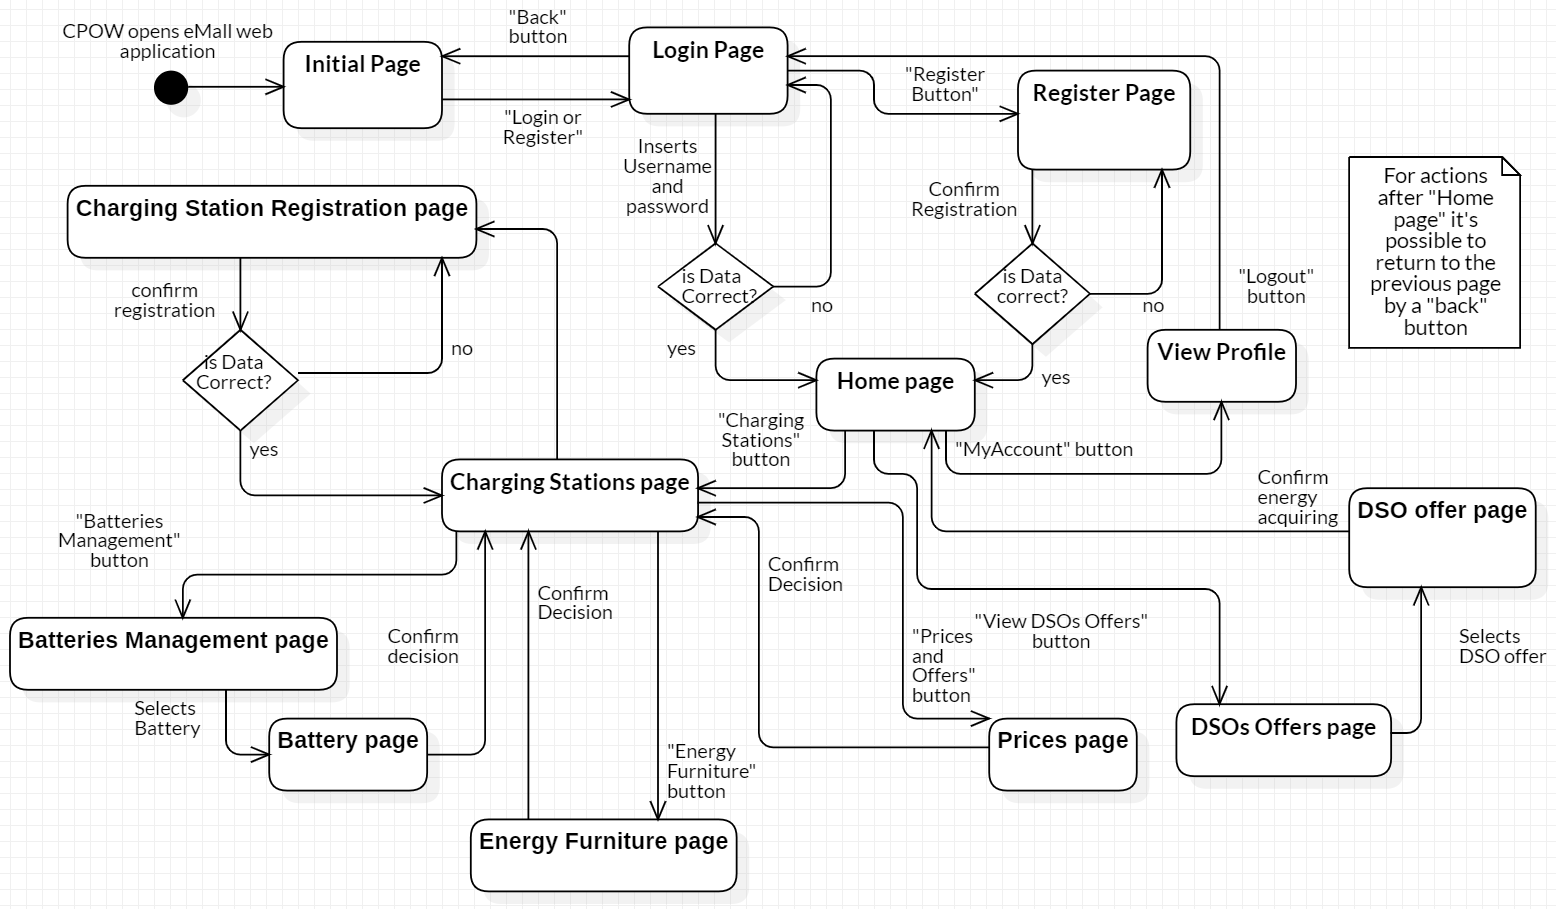
\includegraphics[angle=0, scale=0.7]{img/ACTIVITY DIAGRAM CPOW.png}
\caption{UML Activity Diagram for the CPO Worker Web App navigation}
\label{fig:SupWebApp-activity}
\end{figure}
\end{landscape}
}

\chapter{Requirements Traceability}
In this section is shown how the requirements are actually ensured and which components actually ensure them. It's worth to notice that for the sake of simplicity Mobile Application and eMSP components are considered as one because they work togheter doing the same acrivities, and the Router has been ignored  but it's always involved when dealing with a request coming from one of the clients. 
Table \ref{tab:req-trace} has been added to highlight for each component what requirements it ensures.
\begin{table}[H]  
  \centering
  \begin{tabular}{|c|c|}
    \cline{1-2}
   	\rule{0pt}{10pt} 
   	\begin{large}
    \textbf{Component} 
    \end{large}&\begin{large}
    \textbf{Requirements} 
    \end{large}\\  \hline
    Mobile Application / eMSP &  R1, R2, R3, R5, R6, R7, R8, R9, R10, R11, R12, R13\\ \hline
    Web Application &  R3, R5, R15, R17, R19, R21, R24, R26, R27 \\ \hline
    Notification Manager &  R12, R13\\ \hline
    Access Manager & R3, R4, R5\\ \hline
    Bookings Manager & R9, R10, R11, R14\\ \hline
    Map Manager & R1, R2, R9 \\ \hline
    DSOs Manager &  R19\\ \hline
    Charging Station Manager & R4, R15, R17, R19, R21, R24, R26, R27 \\ \hline
    DataWarehouse & R1, R2, R4, R6, R7, R8, R15, R26, R27 \\ \hline
    
  \end{tabular}
\caption{Table for mapping requirements to components} \label{tab:req-trace}
\end{table}
In the following lines is explained how the requirements are provided by the components:
\begin{itemize}
    \item{[R1]} \label{R1} The system must allow unregistered/registered users to see a map of available charging stations and their prices and offers.
    \item{[R2]} \label{R2} The system must allow unregistered/registered users to see a list of charging stations and filter on it (e.g. offers, prices and positions).
    \item{[R3]} \label{R3} The system must allow unregistered users to register as end user or CPOW (if they have a badge id).
    \item{[R4]} \label{R4} The system must verify if the all data inserted by users are correct (e.g. personal data, vehicle and payment method information, charging station ID).   
    \item{[R5]} \label{R5} The system must allow registered end users or CPOW to log in through their username and password.
    \item{[R6]} \label{R6} The system must allow registered end users to associate vehicles to their account and keep track of them.
    \item{[R7]} \label{R7} The system must allow registered end users to associate payment methods to their account.
    \item{[R8]} \label{R8} The system must allow registered end users to view the available time-slots for a certain type of socket of a certain charging station in a specific day.
    \item{[R9]} \label{R9} The system must allow registered end users to book a charge in a specific charging station.
    \item{[R10]} \label{R10} The system must allow end users to unlock a charging socket if they have booked it and it's the correct time-slot.
    \item{[R11]} \label{R11} The system must let a charge start if a vehicle is correctly connected and the charging socket is unlocked.
    \item{[R12]} \label{R12} The system must show to end users the charging status (e.g. remaining time to complete charge).
    \item{[R13]} \label{R13} The system must notify the end-user when the charge is complete.
    \item{[R14]} \label{R14} When a charging process is correctly finished the system must charge on the end user selected payment system the correct import.
    \item{[R15]} \label{R15} The system must allow CPOW to register a new charging station through its physical id.
    \item{[R16]} \label{R16} The system must be able to dynamically select if using batteries, directly the network or a mix of the two for each charging station.*
    \item{[R17]} \label{R17} The system must allow CPOWs to manually select if using batteries, directly the network or a mix of the two for each charging station associated to them. 
    \item{[R18]} \label{R18} The system must be able to dynamically select which DSO use to provide energy to a specific charging station.*
    \item{[R19]} \label{R19} The system must allow CPOWs to manually select which DSO use to provide energy to a specific charging station associated to them.
    \item{[R20]} \label{R20} The system must be able to dynamically decides if a certain energy furniture is destinated to a battery or directly to sockets of charging stations.*
    \item{[R21]} \label{R21} The system must allow CPOWs to manually decides if a certain energy furniture is destinated to a battery or directly to sockets of charging stations associated to them.
    \item{[R22]} \label{R22} The system must keep track of the current status of each charging process (e.g. booked, startedCharging, etc.).*
    \item{[R23]} \label{R23} The system must keep track of the structure of each charging station (e.g. number of columns, number and type of sockets).*
    \item{[R24]} \label{R24} The system must allow CPOWs to view the structure of each charging station associated to them.
    \item{[R25]} \label{R25} The system must keep track for each charging station of all bookings related to it.*
    \item{[R26]} \label{R26} The system must allow CPOWs to view all the bookings of a certain charging station associated to them and their status.
    \item{[R27]} \label{R27} The system must allow CPOWs to set prices and special offers for a certain charging station associated to him.
\end{itemize}
*R16, R18, R20, R22, R23, R25 requirements refers to the functions done automatically by the CPMS.




\end{document}
